\chapter{Evacuation planning: towards an integrated approach}
\label{ch:evacuation}
% ##################################################################################################################

\hfill \textbf{Author:} Gregor L\"ammel, Christoph Dobler, Hubert Kl\"upfel 

% add a meaningful figure here.
\begin{center} 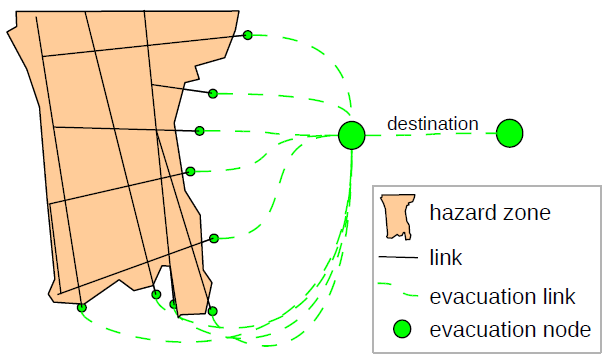
\includegraphics[width=0.4\textwidth, angle=0]{extending/figures/Evacuation/evacuation} \end{center}

This chapter presents an integrated approach for performing evacuation simulations with MATSim.
This integrated approach comprises all steps of the workflow for performing an evacuation analysis, i.e., 
selecting the evacuation area and defining the population, specifiying the behavioral parameters 
(i.e.\ the pre-movement time distribution and the mode of evacuation -- car or pedestrian), 
and analysing the simulation output.
These steps can all be performed within one graphical user interface.
Additionally, two extensions of MATsim for simulating public transport and for changing the network 
during the simulation (i.e.\ network change events) are accessible from the GUI.
In this chapter the steps for performing such an integrated analysis are described and illustrated based on
the example of Hamburg-Wilhelmsburg.

\section{Related work}
\hl{TODO: give references to existing work MATSim related work (e.g./  Diss, Dobler within-day evacuation ...?).
References to other work in the evacuation context are given in Laemmel's Diss - needs to be updated, however.}
Additional work related to evacuation simulations in MATSim is presented by \citet{Dobler_PhDThesis_2013}. The main difference to the approach presented in this chapter is that agents are allowed to adapt their plans on-the-fly using MATSim's within-day replanning framework \citep{DoblerEtAl_TRR_2012}. 
Based on a behavioral model, agents coordinate their actions on household level. If a household is e.g./ not joined when the evacuation starts, each member estimates the time to return home as well as the time to leave the evacuation area directly. Then, the household decides whether meeting at home and leaving together is preferred over every member leaving on its one.
Since the behavioral model is implemented on agent respectively household level, individual attributes such as presence of children in the household or availability of a car can be taken into account.
In contrast to regular MATSim simulations, only a single iteration is performed. Since the agents can optimize their plans continuously using real time information, no further replanning is necessary. As a result, it is guaranteed that agents do not foresee future events such as traffic jams caused by people leaving the threatened area.


%\section{Integrated modeling approach for rapid evacuation planning}
%\hl{TODO: short introduction to GRIPS}
%\section{Input data}
%\hl{TODO: discribe what is needed, where one may get it from, and how it has to transform (if needed).}
%\begin{itemize}
%\item osm file
%\item grips config
%\end{itemize}

\section{Download Matsim and Grips}
Even though it is refered here to the MATSim version \verb|0.6.0-SNAPSHOT| the package should also work with any future version of MATSim.
\begin{enumerate}
\item 
Download the current nightly build of Matsim and Grips from
\url{http://matsim.org/files/builds/}
\item 
Unzip the \verb|Matsim_rxxxxx.zip|, \verb|Matsim_libs.zip| and\\
 \verb|grips-0.6.0-SNAPSHOT-rxxxxx.zip|.
\item 
Move the \verb|grips-0.6.0-SNAPSHOT-rxxxxx.jar| and \verb|libs| folder from the \verb|grips-0.6.0-SNAPSHOT-rxxxxx| directory one level up, 
i.e., to the directory, where \verb|MATSim_rxxxxx.jar| is located.
\end{enumerate}

You can test your configuration by invoking\\ 
\verb|java -cp grips-0.6.0-SNAPSHOT.jar;MATSim_rxxxxx.jar|\\ \verb|org.matsim.contrib.grips.scenariomanager.ScenarioManager|.\\
(You might also want to copy that command to a file \verb|grips.bat| -- or \verb|grips.sh| if using a Unix-like operation system. You can then run that file instead of typing the command.)

\section{The fifteen minute tour}\label{evac:section:fifteenminute}
If you just want to get a quick impression, then the following steps can be performed within a few minutes:
\begin{description}
\item[OSM] Go to \url{www.openstreetmap.org} search for your favorite place and download a (small) osm. Please choose a small area, e.g./ 100m by 100m. This is sufficient for the beginning and the size of the exported area is limited. For larger areas, a direct download from sites like \url{www.geofabrik.de} is preferable (see next section).
\item[Run] the ScenarioManager as described in the previous section.
\item[Create] a scenario by clicking the leftmost button first and then "New". Go to the directory where you'd like to save your project and name the project file (e.g., london.xml or scenario.xml).
\item[Specify] The path of the osm-file (by clicking "Set" next to network), the area ("Set" next to "evacution file") and population files "Set" next to "population file" , and the output directory.
A useful convention is to save everything in the same directory and to name the area file "area.shp" and the population file "population.shp". You can also create sub-directories area and population and save them there.
\textbf{This step has to be done only once. After the scenario-file has been saved, you can just open it in the Scenario-Manager.}
\item[Sample size] Set the sample size to 0.1 (you can use the mouse or the cursor buttons of your keyboard).
\item[Departure] Specify the departure time distribution. Plausible values could be: normal distribution, mu and sigma 600 seconds (10 minutes), earliest 300 seconds, latest 1200 seconds (20 minutes).
\item[Save] your scenario file.
\item[Create] area.shp and population.shp. Currently, the area.shp and population.shp must exist before switching to the area tab. You can download and unzip \url{www.traffgo-ht.com/download/research/grips/shp.zip}. Please make sure all the area and population files (shp, dbf, and some others) are stored in the directory specified in the scenario-file.
\item[Area] Switch to the area tab. You can define the circular evacuation area by keeping the left mouse button pressed and defining the center and radius. Don't forget to save your changes.
\item[Population] Switch to the population tab and define the population (handling is similar to area). Don't forget to save your changes.
\item[Convert] Switch to the next tab and convert the scenario to MATSim input files by clicking the "run" button. The MATSim files will be stored in the output directory specified in the beginning.
\item[Run] the MATSim simulation by skipping the next two tabs/buttons (road closures and busses) and switching to the simulation tab (with the little M for MATSim on the computer screen). Click "run". This will take a while.
\textbf{The output directory will be overwritten. If you want to keep previous results, please rename the output directory.}
\item[Analyze] your simulation results by switching to the final tab after the simulation is finished.

\end{description}

\section{Input data (any place and any size)}
%\hl{TODO: discribe what is needed, where one may get it from, and how it has to transform (if needed).}
The only external input that is necessary for performing an evacuation analysis with \verb|org.matsim.contrib.grips| is an OpenStreetMap file.
You can download OpenStreetMap files from 
\verb+download.geofabrik.de+.
For the sake of this tutorial, we will use the file for Hamburg, Germany. 
Please go to \url{http://download.geofabrik.de/europe/germany/hamburg.html} and download the \verb+hamburg-latest.osm.bz2+ file. This is all the initial preparation you need. Everything else can 
be done with the GUI, called \verb+ScenarioManager+.

\section{Scenario Manager}

The scenario setup, evacuation simulation, and analysis is handled by the so called \verb+ScenarioManager+.
The \verb+ScenarioManager+ is part of the MATSim contribution package \verb+org.matsim.contrib.grips+, where \verb+grips+ stands for GIS-based Risk-Analysis-, Information-, and Planning-System for Regional Evacuation.
The \verb+ScenarioManager+ provides a tool-chain to setup, simulate, and analyze evacuation scenarios.

\subsection{Scenario configuration}


 At start-up the \verb+ScenarioManager+ offers the option to either defining a new scenario configuration or opening an existing one from a XML-file, which then subsequently can be modified. Figure~\ref{chap:evac:fig:sc_man} shows a screenshot of a scenario configuration in the \verb+ScenarioManager+ and the corresponding XML-file respective.


\begin{figure}[!ht]
\begin{subfigure}
\centering
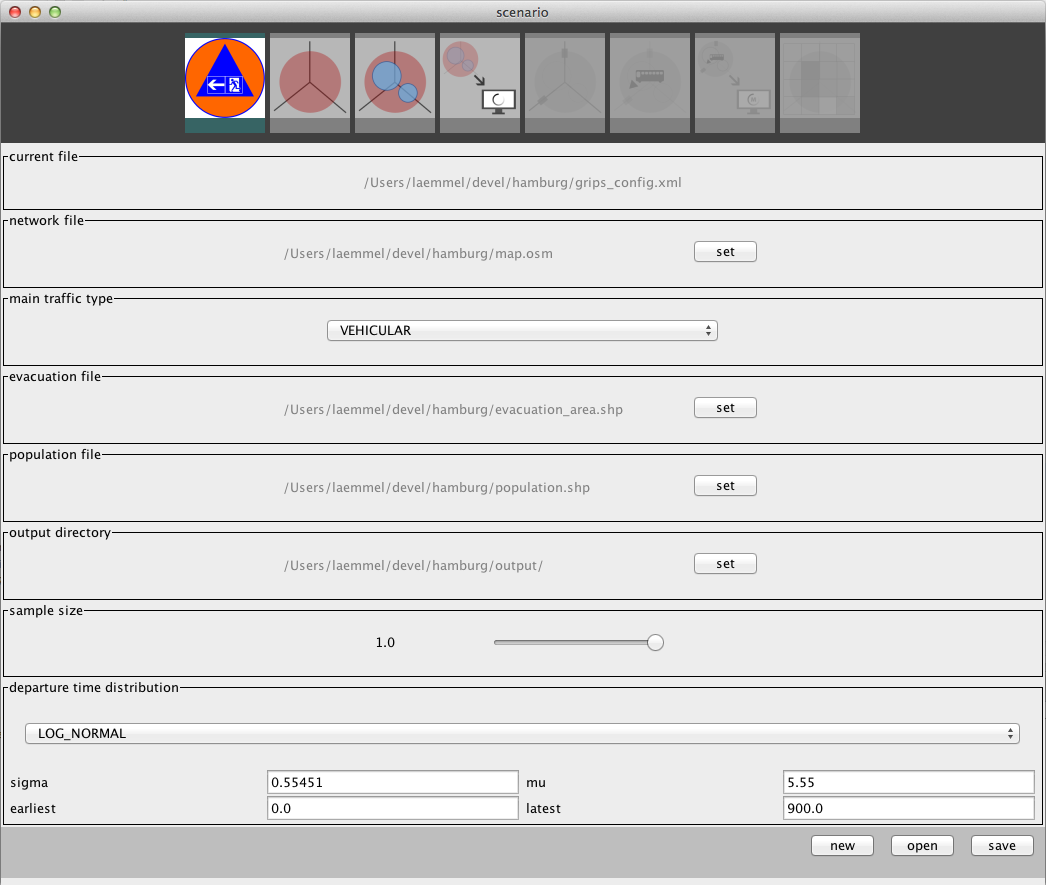
\includegraphics[width=.475\linewidth]{extending/figures/Evacuation/grips_config}
\end{subfigure}\hfill
\begin{subfigure}
\centering
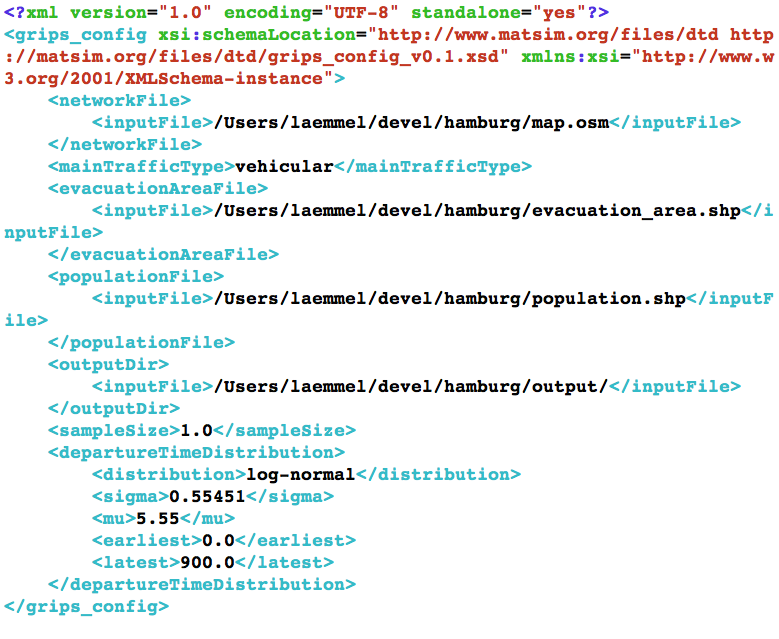
\includegraphics[width=.475\linewidth]{extending/figures/Evacuation/grips_config_xml}
\end{subfigure}
\caption{Illustration of a configurarion opened in the \mbox{ScenarioManager} (left) and as XML-file (right).}\label{chap:evac:fig:sc_man}
\end{figure}
The evacuation scenario is specified by the following parameters:
\begin{itemize}
\item The path to the network file covering the evacuation area. Currently, openstreetmap XML-files are supported (*.osm).
\item The main traffic type for the simulation. This can be either \verb+VEHICULAR+ or \verb+PEDESTRIAN+. Depending on the choice a vehicular specific (the MATSim default) or a pedestrian specific (as discussed in~\citet{LaemmelKluepfelNagel2009EvacPadangAtBookTimmermanns,Laemmel_PhDThesis_2011}) simulation network will be generated by setting free spee, number of lanes, and flow capacity for the links in the network accordingly.
\item The path to an ESRI-Shape file describing the extend of the evacuation area by a simple polygon. This file does not need to be exist right from the beginning but can be produced manually by the \verb+ScenarioManager+ itself as discussed later.
\item The path to an ESRI-Shape file giving the size and distribution of the affected population. This file comprise a set of simple polygons with each polygon has an additional attribute for the number of persons residing at a location inside that polygon. As for the evacuation area this file can be produced with help of the  \verb+ScenarioManager+.
\item The path to the output directory where the simulation output and MATSim scenario files will be stored.
\item The sample size for the MATSim simulation. A smaller sample size increases the simulation performance, while a larger size might increase accuracy of the results. Typical values are 1.0, 0.1, or 0.01 depending on the scenario and the available computing resources.
\item The departure time distribution defines the distribution from which the departure times for the simulation will be drawn. The intention behind this is that in real evacuation situations it is not expected that all people start simultaneously with their evacuation. 
People tent to perform pre-evacuation activities before they start. Those activities include picking up relatives, to pack food, cloths, or valuable belongings, and other things. 
Since number and duration of those activities differs on the individual level the departure times of the population is an unknown quantity. The \verb+ScenarioManager+ supports three different distributions (Dirac-delta, normal, and log-normal). If the user choses the Dirac-delta distribution then all evacuees will start at once, which might be the worst case~\citep{LaemmelKluepfel2012InfluenceOfDepartureTimeDistribution}. By choosing the normal distribution the departure times for the individuals are drawn from a normal distribution with mean $\mu$ and standard deviation $\sigma$, where the parameters $\mu$ and $\sigma$ are of unit [second]. As an example, setting $\mu = 1800$ and $\sigma =  900$ will result in a departure time distribution where on average after 30 min 50\% of the population has departed and 68.3\% of the population departs in the time interval of 30 min $\pm$ 15 min. If the user decides to choose log-normal as the distribution then the departure times are drawn from a log-normal distribution, where $\mu$ and $\sigma$ are the parameters of the associated normal distribution (a discussion on this matter is given below). The parameters \emph{earliest} and \emph{latest} determine the earliest and latest possible departure time. The normal and log-normal departure time distribution are truncated accordingly.
\end{itemize}
The departure time distribution is maybe the most unclear parameter to set. The authors are not aware of any holistic research into this matter. 
In general, it seems to be reasonable to assume that a lot of people starting the evacuation at about the same time soon after the evacuation order has been issued and as the the time proceeds fewer and fewer people still have to depart. 
This calls for a departure time distribution that has a probability density function with a steep positive gradient at the beginning and after a peak it levels out slowly. The probability density function of a log-normal distribution produces this kind of curve. log-normal and normal distributions are closely related. If the random variable $Y$ is normal distributed, then $X = \text{exp}(Y)$ is log-normal distributed. The expected value $E[X]$  and the variance $Var[X]$ are
\begin{equation}
E[X] = \text{exp}(\mu + \frac{\sigma^2}{2})
\end{equation}
and 
\begin{equation}
Var[X]=\text{exp}(2(\mu+\sigma^2))-\text{exp}(2\mu+\sigma^2).
\end{equation}
Conversely, if the expected value and variance is given $\mu$ and $\sigma$ of the associated normal distribution can be obtained as follows:
\begin{equation}
\sigma = \sqrt{\text{log}(1+\frac{Var[X]}{(E[X])^2}}\label{chap:evac:eq:sigma}
\end{equation}
and 
\begin{equation}
\mu = \text{log}(E[X] - \frac{1}{2}\sigma^2).\label{chap:evac:eq:mu}
\end{equation}
If the users wishes to generate a population with departure times that follow a log-normal distribution it is hard to see how $\sigma$ and $\mu$ will determine the outcome. It is much more convenient to think about the expected value and variance. Given Equations~(\ref{chap:evac:eq:sigma}) and (\ref{chap:evac:eq:mu}) a conversion from expected value and variance to $\sigma$ and $\mu$ is straightforward.

\subsection{Evacuation area}% and population}
The \verb+ScenarioManager+ integrate a modules for the definition of the evacuation area and the distribution of the affected population. The so called evacuation area selection module allows the user to define the evacuation area by drawing either a simple polygon or a circle on map. The application can make use of either a WMS-provider or a tile map provider (e.g./ openstreetmap) as background map renderer. Zooming and panning is restricted to the bounding box of the openstreetmap network file provided in the scenario configuration. An illustration of the evacuation area selector is given in Figure~\ref{chap:evac:fig:area_pop}. Besides defining a new evacuation area a pre-existing one can also be loaded into the \verb+ScenarioManager+. The requirements to a pre-existing evacuation area file are:
\begin{itemize}
\item It has to be provided as a ESRI-Shape file.
\item The evacuation area must be defined as a simple polygon or a multi-polygon that contains one and only one simple polygon.
\item The coordinate reference system for polygon in the ESRI-Shape file has to be set correctly. 
\end{itemize}
However, due to the error-proneness of this approach it is only recommended for experienced users.

Later in the process the \verb+ScenarioManager+ takes the evacuation area to cut out an evacuation network. However, after cutting out the evacuation net there is no particular node as a target for the path
calculation, as the evacuees have more than one safe place to evacuate to. Instead,
in the underlying domain every node outside the evacuation area is a possible
destination for an evacuee that is looking for an escape route. Thus, the evacuation problem is in general a multi-destination problem. To resolve this,
the standard approach (e.g.~\citet{FordFulkerson1962FlowsInNetworks,LuGeorgeEtAl2005CapacityConstrainedRouting})
is to extend the network in the following way: All exit links (i.e.\ links that are originating inside the evacuation area and terminating outside the evacuation area) are connected, using virtual links with infinite flow capacity
and zero length, to a super-node, and all evacuation paths are routed to the super-node. This way, the problem is reduced to a multi-source single-destination problem. And thus, finding the shortest path from any node inside the evacuation area to this super-node and, in consequence, to safety can efficiently be solved.


\subsection{Evacuation demand}
The process of defining the population distribution is similar to that of the evacuation area. 
The difference is that the population is distributed over circles drawn on the map. 
The user can draw an arbitrary number of those circles and define for each circle the population figures individually. Figure~\ref{chap:evac:fig:area_pop} illustrates the population editor. 
\begin{figure}[!ht]
\begin{subfigure}
\centering
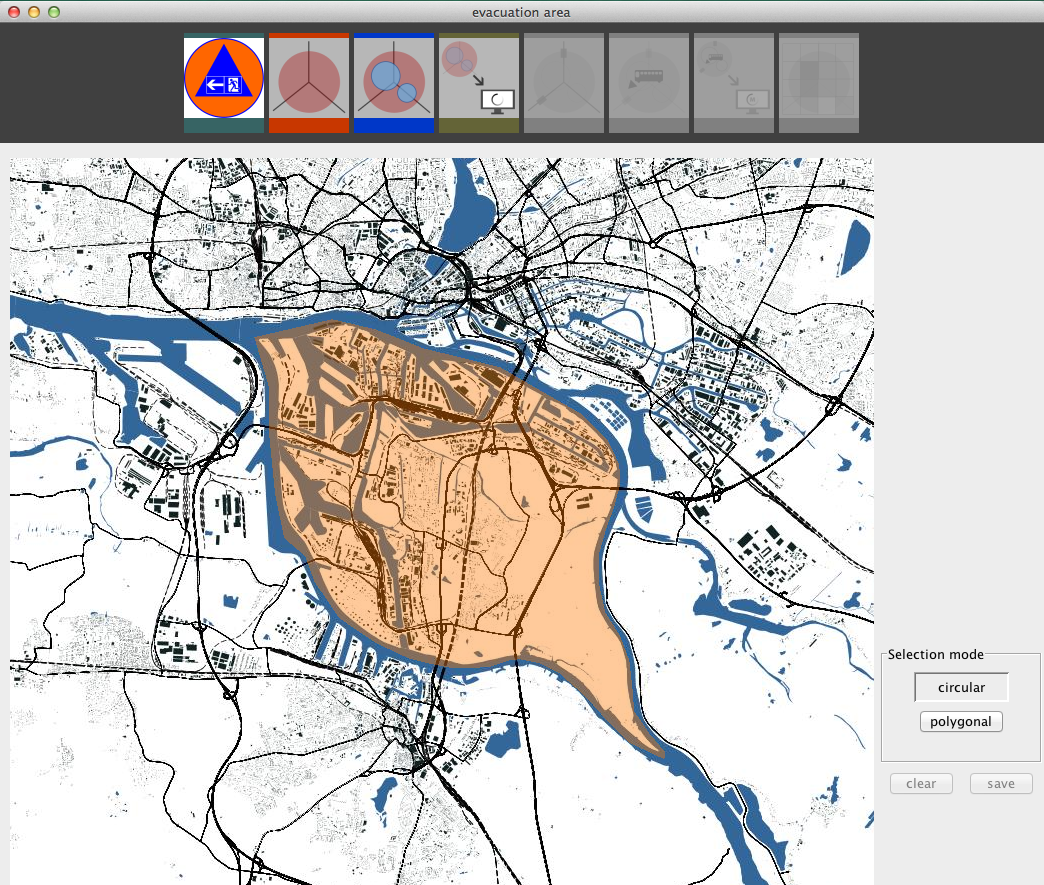
\includegraphics[width=.475\linewidth]{extending/figures/Evacuation/evac_area_sel}
\end{subfigure}\hfill
\begin{subfigure}
\centering
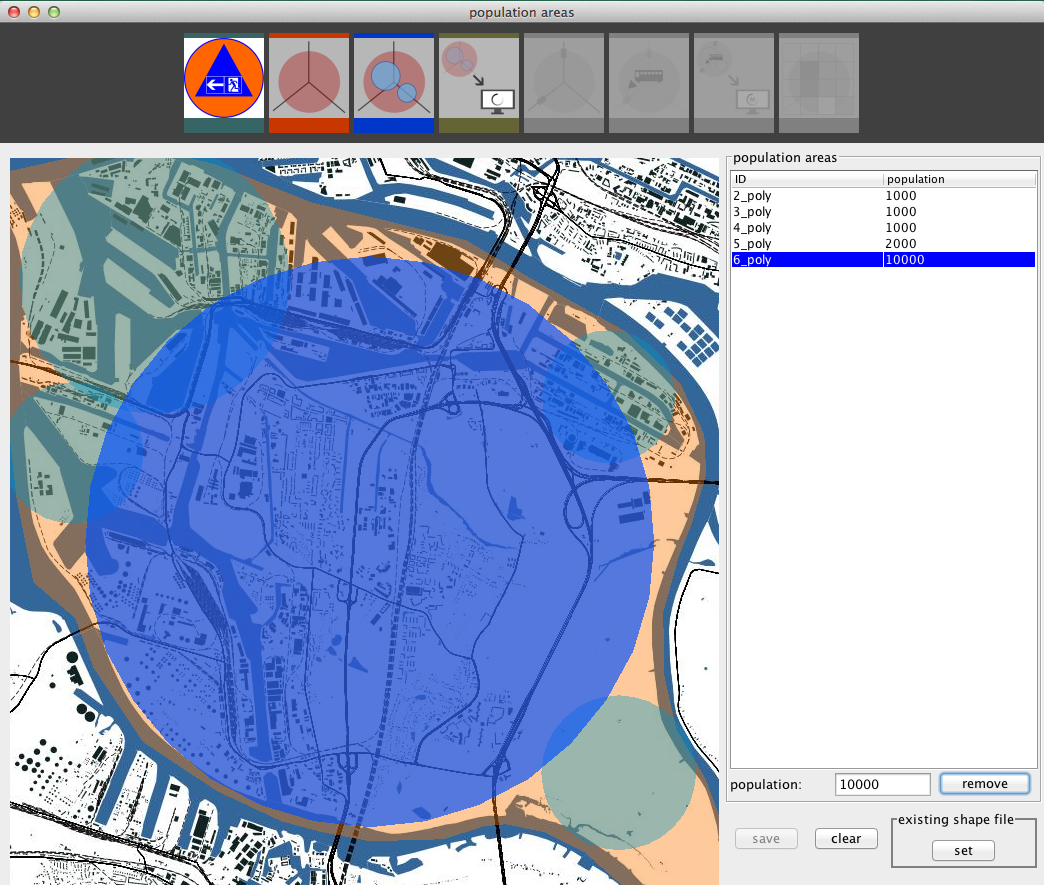
\includegraphics[width=.475\linewidth]{extending/figures/Evacuation/pop_sel}
\end{subfigure}
\caption{The evacuation area (left) and the population distribution (right) can be defined with an integrated GIS application.}\label{chap:evac:fig:area_pop}
\end{figure}
The population editor only offers basic functionality to define a population distribution. For every circular area the \verb+ScenarioManager+ produces as many agent as requested and assigns for each agent a random coordinate inside the circular area. However, in MATSim agents depart on links so the \verb+ScenarioManager+ calls the \verb+getNearestLink()+ method defined in \verb+NetworkImpl+. Thus, agents will depart on links inside and possibly nearby the circular areas. 

In the current version it is not possible to use a predefined demand for the simulation. Extending the simulation package in this way would be straightforward but is out of scope of this work.


\subsection{Road closures}
In real situations it is often the case that not all exiting roads are available for the evacuation. This might be for several reasons:
\begin{itemize}
\item They might be impassable due to the event. This is often the case in flooding related evacuations.
\item The authorities might want to keep roads open exclusively for action forces.
\item In some situations, like hurricane evacuations, the direction of lanes on motorways might be reversed to in crease the flow capacity in one direction.
\item The authorities have detailed evacuation plans in place with pre-planned evacuation routes and so road closures might become necessary in order to force evacuees to take this routes.

\end{itemize}
The actual planning of road closures can be a complex undertaking and not all attributes of such a planning can be integrated in a simple tool for rapid evacuation planning. Nevertheless, the  \verb+ScenarioManager+ offers a tool for editing of time-dependent road closures. An illustration of the road closures editor is given in Figure~\ref{chap:evac:fig:rd_closures_bus_stops}.
\begin{figure}
\begin{subfigure}
\centering
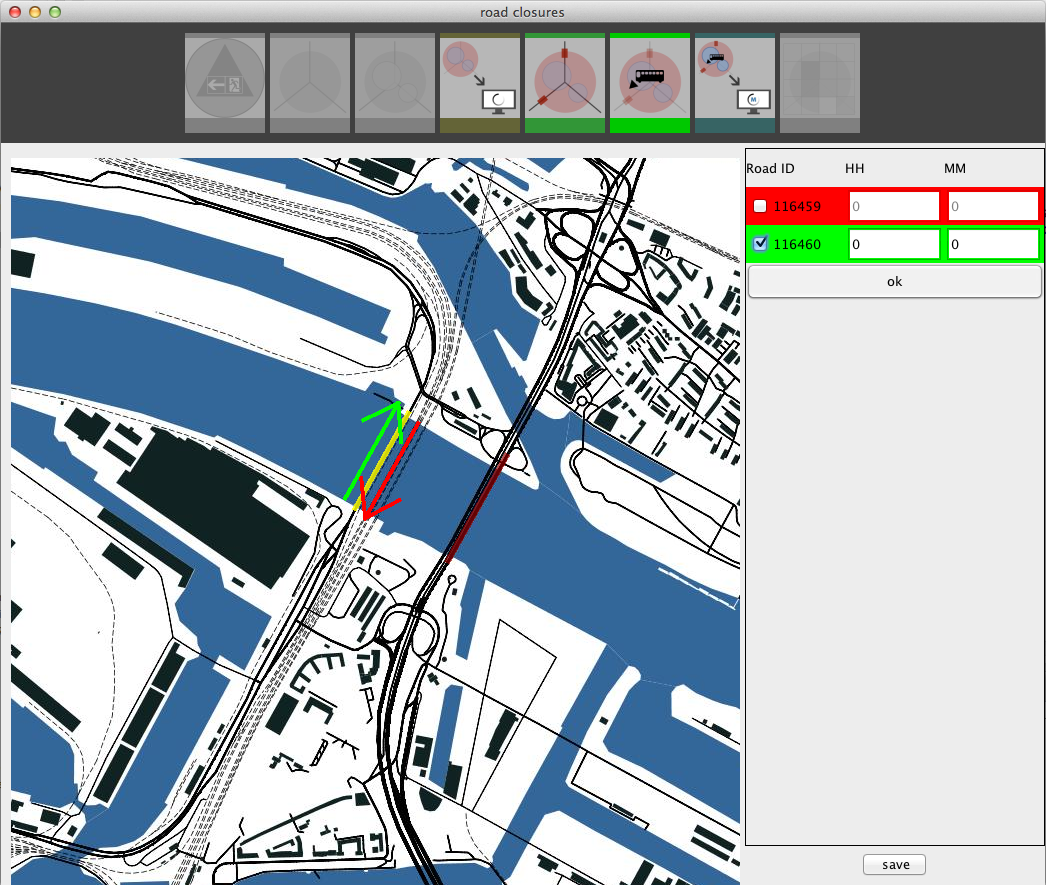
\includegraphics[width=.475\linewidth]{extending/figures/Evacuation/rd_closure_detail}
\end{subfigure}\hfill
\begin{subfigure}
\centering
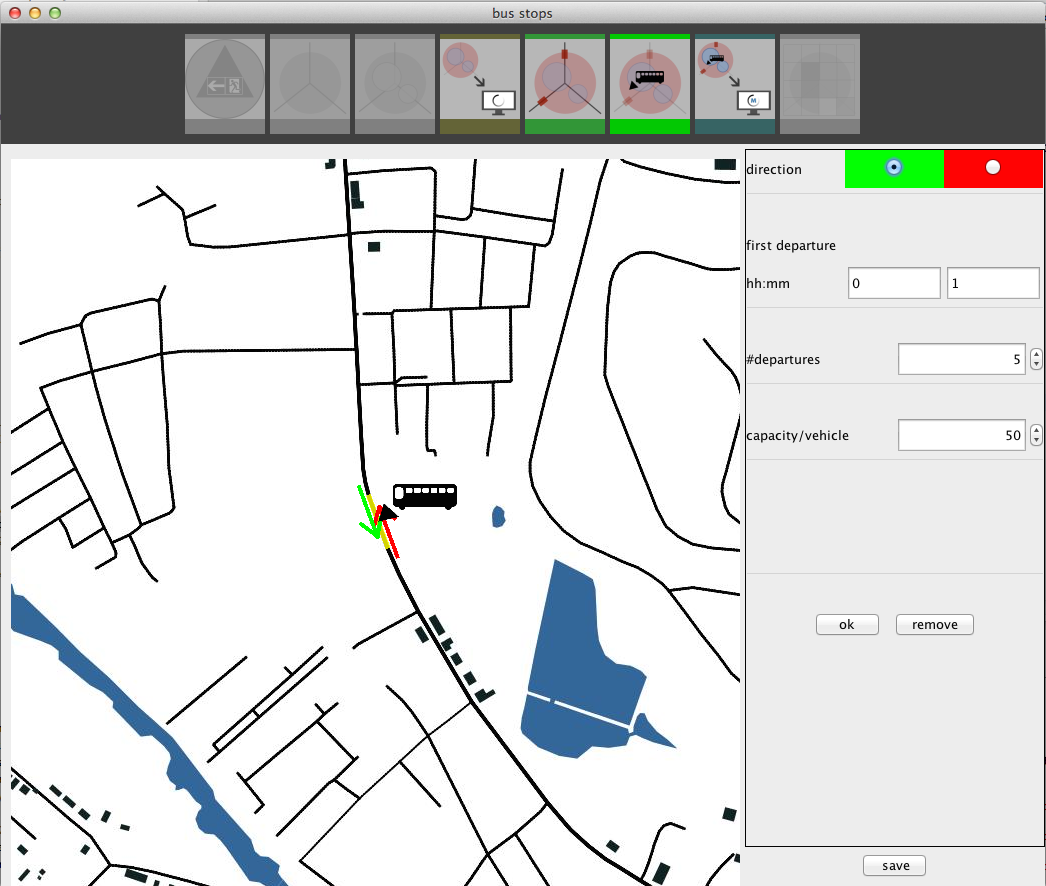
\includegraphics[width=.475\linewidth]{extending/figures/Evacuation/bus_stops}
\end{subfigure}
\caption{Left: Road closures can be edited by an integrated GIS application. For every link the direction and the time of closure can be defined. Right: Tool that let the user define bus stop locations and schedules }\label{chap:evac:fig:rd_closures_bus_stops}
\end{figure}
Road closures are stored as \verb+NetworkChangeEvents+ and handled as time-dependent network attributes in MATSim.

\subsection{Bus stop editor}
Usually not all people have access to a private car. In the event of an evacuation those people often rely on public transport. What is more, in region that are prone for natural disasters the local authorities normally have detailed evacuation plans in place. Those plans might include the evacuation by public transport. Consequently, it is of great interest to have a tool available that helps with the integration of public transport into to the simulation framework. The \verb+ScenarioManger+ offers this possibility by defining bus stops and bus schedules in the interactive GUI. Figure~\ref{chap:evac:fig:rd_closures_bus_stops} gives an example of the bus stop editor. Besides the location the user can define when the first bus will serve this bus stop, how many busses overall will serve this particular bus stop, and of what capacity those busses are. 
The \verb+ScenarioManager+ transforms the inputs made in the GUI into a MATSim compatible transport schedule. This means it enriches the scenario while using the same simulation model as before. Details about public transport simulations with MATSim are given in Chapter~\ref{ch:pt}. A tutorial can be found on the MATSim webpage (\verb+http://matsim.org/docs/tutorials/transit+).
Limitations of the public transport evacuation approach in this project are:
\begin{itemize}
\item Each bus serves one and only one bus stop, which might be not too unrealistic either.
\item Busses alway take the shortest path from their designated bus stops to the safe area. As the shortest path is not necessarily the fastest path this approach might lead to avoidable delays. Some newer research investigate the optimization of bus lines with respect to traffic demand and traffic condition~\citep{Neumann_PhDThesis_2014}. Implementing such optimization techniques int the evacuation context is a topic of future research.
\end{itemize}

\subsection{Running the scenario}
The \verb+ScenarioManager+ runs the evacuation simulation in similar way it is done in other transport simulation studies with MATSim. 
At the beginning an evacuation plan is assigned to each evacuee. 
An evacuation plan describes the way how the evacuee intents to reach the safe area.
In Case the evacuee evacuates by car or foot then such a plan essentially comprise a route (typically the shortest route) from home to the safe area. For evacuees who are evacuating by public transport such a plan can be much more complex. All those evacuation plans will be executed in the mobility simulation. After the mobility simulation terminates all plans are scored regarding their resulting travel time. 
As shorter a plan's resulting travel time is as higher is the score it receives. After this step the evacuees' plans are revised some evacuees will receive new plans while others will stick with the current ones. This step is called re-planning. Mobility simulation, scoring, and re-planning are repeated in a loop for a predefined number of iterations. The evacuees' individual performance improve over the iterations. 
In general transport studies this approach is meant to emulate the real-world travelers behavior when they perform their daily commutes and try to find better travel alternatives. Evacuations, however, are singular events where such a day-to-day re-panning would not occur. We argue here that the chosen iterative learning approach could be seen as the evacuees anticipation of the conditions that are expected during an evacuation. 
Since people who know their  environment would likely avoid roads that obviously constitute bottlenecks during an evacuation. Nevertheless, there is more research needed in order to get a definitive answer how people choose evacuation routes or how many iterations of learning are realistic to reflect the assumed anticipation skills adequately. As a rule of thumb, running 100 iterations of learning are usually enough to get results the constitute a lower boundary in terms of resulting evacuation times.
This is only a rough description of the iterative learning frame work. Details about the general framework are discussed in Chapter~\ref{ec:co-ev}. Deeper insights into evacuation planning with MATSim can be found in~\citep{Laemmel_PhDThesis_2011}.

\subsection{Analysis}
After the last iteration has finished the \verb+ScenrioManager+ enables the analysis module. The analysis modele evaluates the performed simulation run by a number of different methods. 
\begin{itemize}
\item The cumulated arrival curve tells the user the number of evacuated persons over time. From this curve the user can for example read at what time 50\% of the population are in safety.
\item The GIS based evacuation time analysis draws a grid over the evacuation area and computes for every grid cell the average evacuation time. The evacuation times are indicated be different colors. Therefor, the analysis modules runs a quantiles-based clustering analysis for each cell. The size of the cells can be varied  by the user.
\item The GIS based clearance time analysis is performed in the same way as the evacuation time  analysis. The clearance time of a cell is the time when the last evacuee leaves that cell. This evacuee is not necessary one who also started her evacuation inside the corresponding cell but might also be one who crosses that cell somewhen during the evacuation.
\item A similar quantiles-based clustering approach is used for the link utilization analysis. The link utilization analysis results help the user to identify the roads with the highest utilization during the evacuation.
\end{itemize}
The analyses can be run for every single iteration for which the MATSim controller has dumped an events file. By default this every 10th iteration. An overview of the analysis module is given in Figure~\ref{chap:evac:fig:analysis}
\begin{figure}
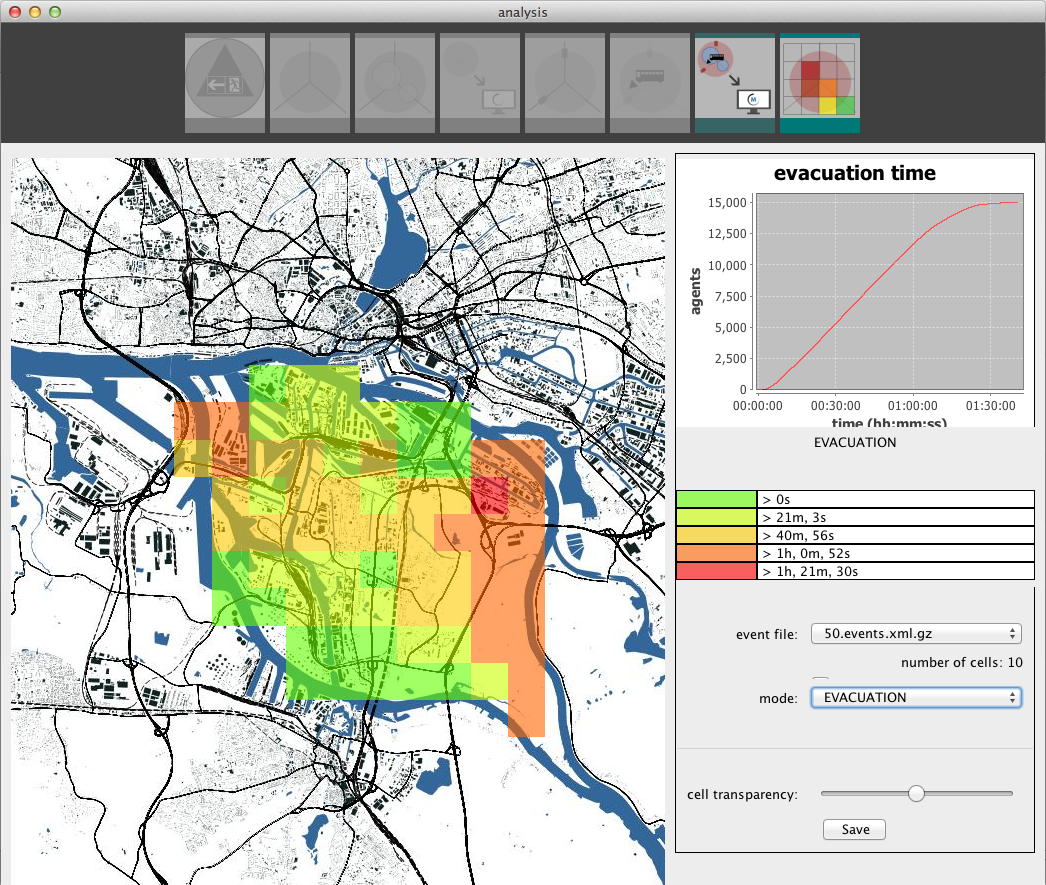
\includegraphics[width=1\textwidth]{extending/figures/Evacuation/it50_evac_time}
\caption{Screenshot of the analysis module showing GIS based evacuation time analysis and the evacuation curve.}\label{chap:evac:fig:analysis}
\end{figure}

\section{Conclusion}
